\documentclass[11pt,a4paper]{ctexart}
\usepackage[margin=2.4cm]{geometry}
\usepackage{graphicx}
\usepackage{booktabs}
\usepackage{amsmath}
\usepackage{amssymb}
\usepackage{hyperref}
\usepackage{enumitem}

\title{同轴显微成像下反光表面缺陷形貌的眩光感知焦栈重建方法：光学机理报告骨架}
\author{SRTP Project Notes}
\date{2026-06-21}

\begin{document}
\maketitle

\begin{abstract}
本文档总结反光工业表面缺陷焦栈三维重建中的核心光学问题。初步焦堆诊断显示，部分真实样本在若干焦层中存在局部高亮和近饱和现象，且这些高亮层可能与传统 Laplacian/Tenengrad 焦点评价峰重合。本文建议将投稿主线收束为 flare-aware focus-stack reconstruction：首先从同轴照明、局部法线、物镜接收孔径和离焦点扩散解释 DFF 失效，再用微米级仿真高度图构造 glare-risk prior 与合成 ground truth，最后通过先验引导网络提升反光缺陷形貌重建稳定性。
\end{abstract}

\section{Problem Statement}

传统 depth from focus (DFF) 假设每个像素在真实焦平面附近具有最强清晰度响应。然而在同轴显微成像下，反光微结构可能产生局部高亮、近饱和和离焦亮斑边缘，使 focus measure 的最大值偏离真实高度。本文建议围绕如下问题组织投稿：

\begin{quote}
How can focus-stack reconstruction remain stable when reflective microstructures generate glare-induced focus artifacts under coaxial microscopy?
\end{quote}

\section{Preliminary Evidence}

本轮分析对 6 组真实焦堆做了轻量统计。最强证据来自 \texttt{钥匙纹路100um}：该样本有 40 个焦层，最大近饱和比例约为 0.0126，任一焦层高亮比例约为 0.0520，Laplacian 最强焦层位于第 2 层。低眩光对照样本 \texttt{3D表面} 和 \texttt{3D层纹} 没有明显近饱和像素，焦点评价峰更接近正常对焦响应。

\begin{figure}[htbp]
  \centering
  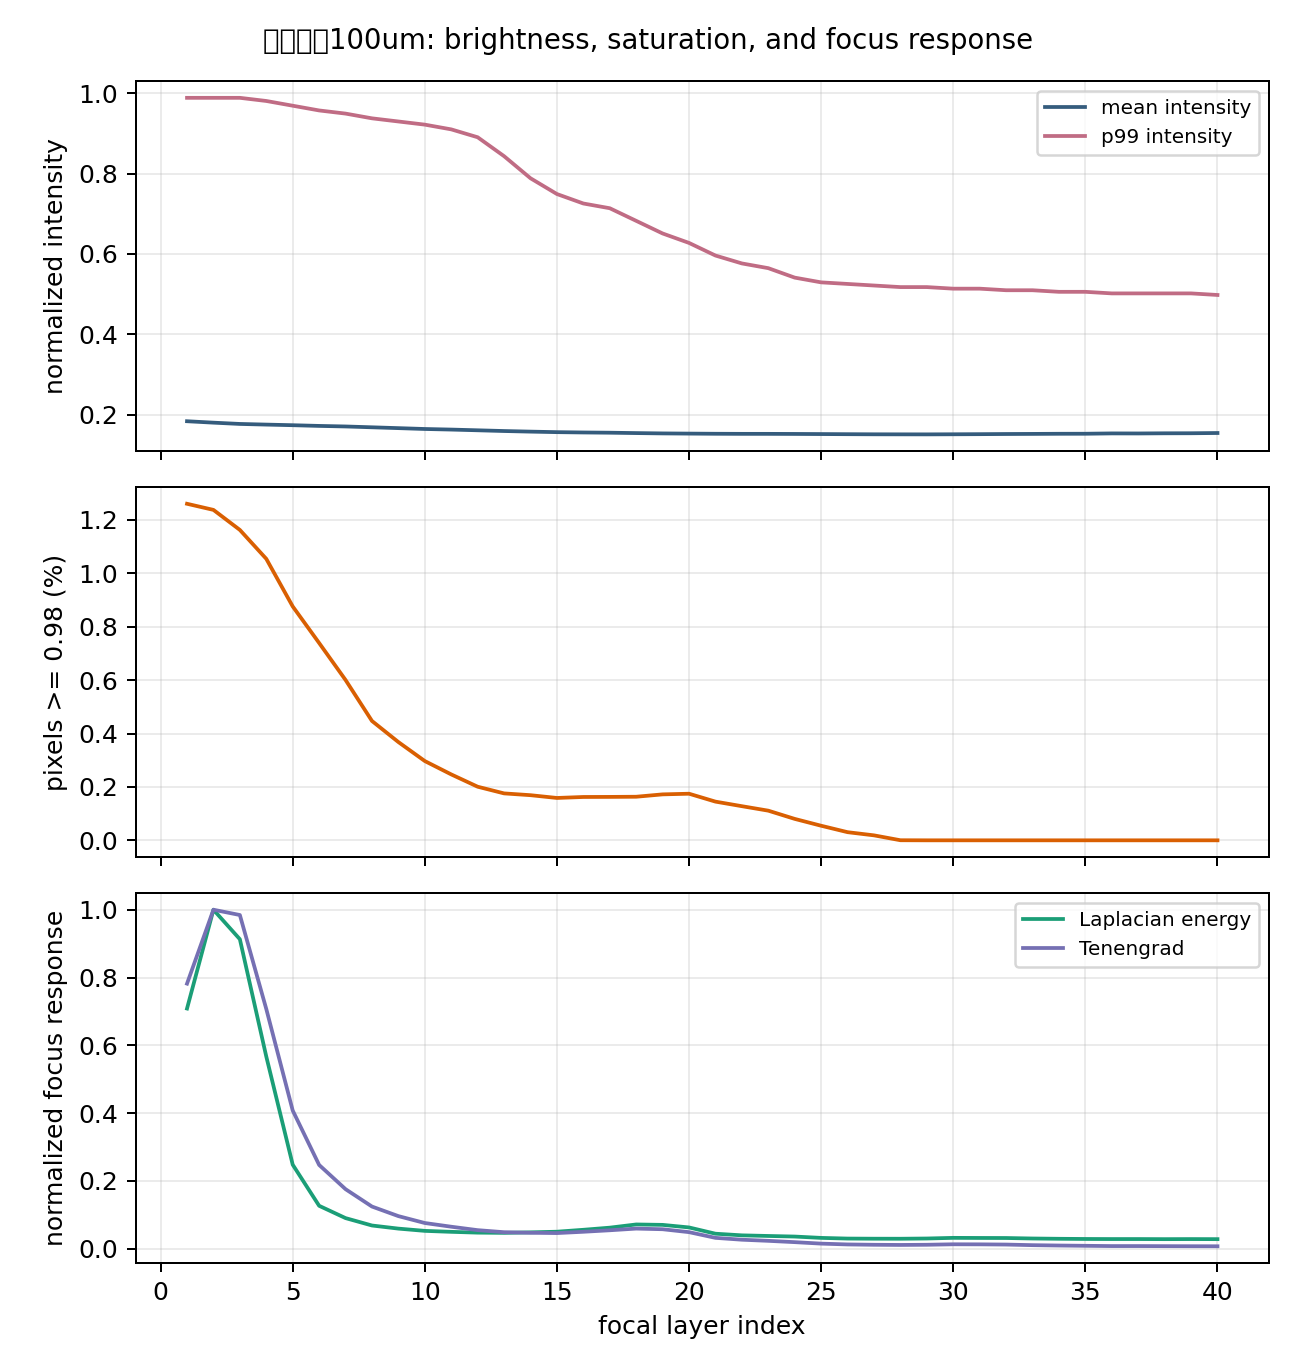
\includegraphics[width=0.95\linewidth]{figures/钥匙纹路100um_curves.png}
  \caption{高反光样本的亮度、近饱和比例与焦点评价曲线。}
  \label{fig:keycurve}
\end{figure}

\begin{figure}[htbp]
  \centering
  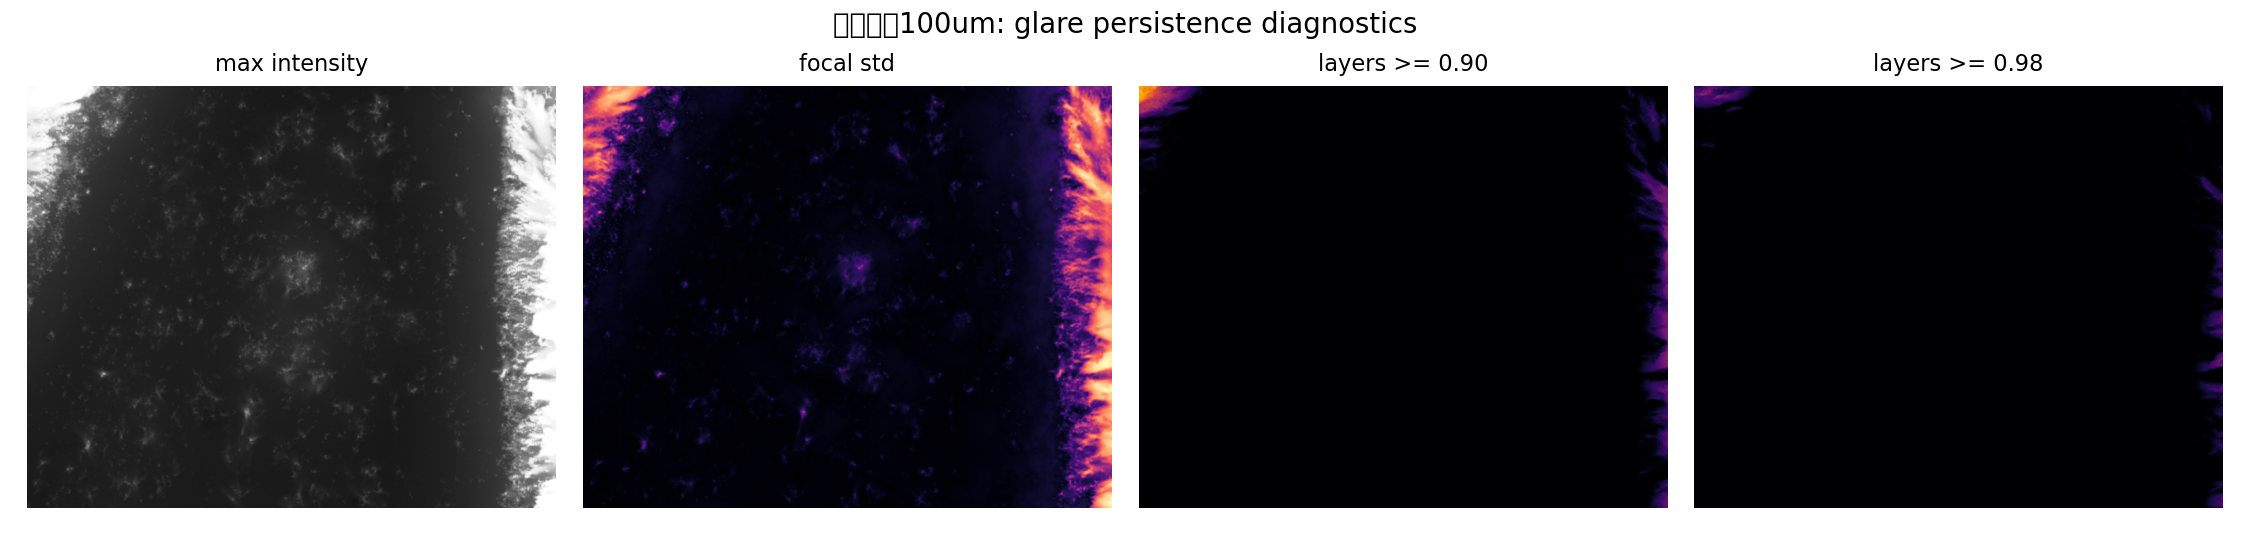
\includegraphics[width=0.95\linewidth]{figures/钥匙纹路100um_persistence.png}
  \caption{高反光样本的跨焦层高亮持久性图。}
  \label{fig:keypersistence}
\end{figure}

\section{Optical Mechanism}

\subsection{Normal-Aperture Matching}

设局部法线为 $\mathbf{n}$，入射方向为 $\mathbf{l}$，观察方向为 $\mathbf{v}$。镜面反射方向可写为：
\begin{equation}
\mathbf{r}=2(\mathbf{n}\cdot\mathbf{l})\mathbf{n}-\mathbf{l}.
\end{equation}

若反射方向进入物镜接收锥，则该位置具有较高眩光风险：
\begin{equation}
G(\mathbf{x})=\mathbb{I}\left[\arccos(\mathbf{r}\cdot\mathbf{v}) \leq \theta_{\mathrm{obj}}\right],
\quad
\theta_{\mathrm{obj}}=\arcsin\left(\frac{\mathrm{NA}}{n_{\mathrm{medium}}}\right).
\end{equation}

在空气中 $n_{\mathrm{medium}}\approx 1$，若 $\mathrm{NA}=0.4$，则 $\theta_{\mathrm{obj}}\approx 23.6^\circ$。该表达式提供了从高度图、法线场到 glare-risk map 的最小物理模型。

\subsection{Defocused Highlight Edges}

焦层 $k$ 的观测图像可近似写为：
\begin{equation}
I_k(\mathbf{x})=\mathrm{clip}\left( h_k(\Delta z) * R(\mathbf{x},\mathbf{n},\mathbf{l},\mathbf{v}) + \epsilon \right),
\end{equation}
其中 $h_k$ 是与离焦量相关的点扩散函数，$R$ 是反射亮度项，$\epsilon$ 是噪声。传统焦点评价可抽象为：
\begin{equation}
F_k(\mathbf{x})=\Phi\left(I_k(\Omega_{\mathbf{x}})\right).
\end{equation}

当局部高亮被饱和截断，亮斑平台边界仍会产生强梯度或高 Laplacian 响应，使 $\arg\max_k F_k(\mathbf{x})$ 偏向高亮层。

\subsection{Recoverable and Unrecoverable Glare}

给定阈值 $\tau$，定义跨焦层饱和持久性：
\begin{equation}
P_{\tau}(\mathbf{x})=\frac{1}{K}\sum_{k=1}^{K}\mathbb{I}[I_k(\mathbf{x})\geq\tau].
\end{equation}

$0<P_{\tau}(\mathbf{x})<1$ 的区域可能仍有部分焦层保留可恢复纹理；$P_{\tau}(\mathbf{x})\approx1$ 的区域则高度依赖邻域结构或低置信度输出。该定义可直接用于分区评估和模型 prior。

\section{Proposed Storyline}

建议暂定题目为：

\begin{quote}
\textbf{Flare-Aware Focus-Stack Reconstruction for Reflective Surface Defect Morphology under Coaxial Microscopy}
\end{quote}

建议贡献点包括：

\begin{enumerate}[leftmargin=2em]
  \item 分析反光微结构、同轴照明和物镜接收孔径如何导致 DFF focus artifacts。
  \item 构造基于高度图、法线和接收锥的 glare-risk simulation engine。
  \item 将 DFF/GADFF、focal-difference、saturation persistence 和 glare-risk map 输入统一的先验引导模型。
  \item 区分 synthetic quantitative evaluation 与 real no-reference morphology validation。
\end{enumerate}

\section{Related Work Matrix}

\begin{table}[htbp]
\centering
\small
\begin{tabular}{p{3cm}p{4cm}p{6cm}}
\toprule
Theme & Representative Works & Use in This Paper \\
\midrule
Classical SFF/DFF & Nayar1994; Pertuz2013; Lee2013; Li2019 & Establish interpretable focus measures and traditional baselines. \\
Learning-based DFF & DDFFNet; AiFDepthNet; DFV; DfF in the Wild; DDFS & Provide main external baselines and focal-volume modeling references. \\
Defocus / Sim-to-Real & Focus on Defocus; DEReD; Dr.Bokeh & Support optical modeling, self-supervision, and differentiable defocus rendering. \\
Industrial 3D Defect & Att-PU-Net BDSIM & Position the task in quantitative optical surface-defect reconstruction. \\
Depth Foundation Models & Depth Anything; Depth Anything V2 & Support synthetic labels and pseudo-labeled real data as training strategy references. \\
\bottomrule
\end{tabular}
\caption{Recommended related-work organization.}
\end{table}

\section{Experiment Plan}

\begin{enumerate}[leftmargin=2em]
  \item 对真实焦堆输出 ROI 级亮度曲线、饱和持久性图和 focus response 曲线。
  \item 建立微高度图法线-孔径仿真，输出 glare-risk map。
  \item 在合成数据中按 glare-risk 区域报告 MAE、edge MAE 和 high-risk MAE。
  \item 统一最终模型为 Flare-FocusNet 或 Flare-Aware Focus-ResUNet。
  \item 优先适配 DFV 和 DDFFNet 作为 learning-based baselines。
  \item 若条件允许，用 WLI、共聚焦或 step-height 标准样补充小规模真实高度真值。
\end{enumerate}

\section{References}

\begin{itemize}[leftmargin=2em]
  \item Nayar and Nakagawa, ``Shape from focus,'' IEEE TPAMI, 1994. \url{https://doi.org/10.1109/34.308479}
  \item Pertuz et al., ``Analysis of focus measure operators for shape-from-focus,'' Pattern Recognition, 2013. \url{https://doi.org/10.1016/j.patcog.2012.11.011}
  \item Yang et al., ``Deep Depth from Focus with Differential Focus Volume,'' CVPR, 2022. \url{https://arxiv.org/abs/2112.01712}
  \item Won and Jeon, ``Learning Depth from Focus in the Wild,'' ECCV, 2022. \url{https://arxiv.org/abs/2207.09658}
  \item Fujimura et al., ``Deep Depth from Focal Stack with Defocus Model for Camera-Setting Invariance,'' IJCV, 2024. \url{https://arxiv.org/abs/2202.13055}
  \item Nikon MicroscopyU, ``Numerical Aperture.'' \url{https://www.microscopyu.com/microscopy-basics/numerical-aperture}
  \item Wang et al., ``Defect 3D reconstruction with integrated bright-field and dark-field structured illumination microscopy based on Att-PU-Net,'' Applied Optics, 2026. \url{https://doi.org/10.1364/AO.587592}
\end{itemize}

\end{document}
